\documentclass[fontsize=13pt,a5paper,twoside, DIV=calc]{scrbook}
\usepackage[ngerman]{babel}
\usepackage[no-math]{fontspec}
\usepackage{microtype}
\setmainfont[
 BoldFont={Merriweather Bold}, 
 ItalicFont={Merriweather Italic Italic},
 BoldItalicFont={Merriweather Italic Bold Italic}
 ]{Merriweather}
\setsansfont[
 BoldFont={Merriweather Sans Bold}, 
 ItalicFont={Merriweather Sans Italic},
 BoldItalicFont={Merriweather Sans Bold Italic}
 ]{Merriweather Sans}
\setmonofont{FreeMono}
\newfontface\FontB{Noto Sans Hebrew}
\newfontface\FontC{Noto Sans Tamil}
\newfontface\FontD{Noto Sans Thai}
\newfontface\FontE{Noto Sans Georgian}
\newfontface\FontF{Noto Sans Devanagari}
\newfontface\FontG{Noto Sans CJK JP}
\newfontface\FontH{Noto Sans Arabic}
\newfontface\FontI{Noto Sans Yi}
%Ermöglicht Zierkapitälchen zum Anbsatzanfang
\usepackage{lettrine}
\input Kramer.fd
\newfontface\FontJ{Kramer}
\renewcommand{\LettrineFontHook}{\color{farbe}\relax\FontJ}
%Hiroglyphen
\usepackage{hieroglf}
%Für kapitel Zahlen
\usepackage{amsmath}
\usepackage{mathspec}
\setmathfont(Digits,Latin)[Scale=MatchLowercase]{Merriweather}
%Erlaubt Einsatz von Farbe
\usepackage[svgnames]{xcolor}
\definecolor{farbe}{HTML}{766D20}
%UTF 8
%\usepackage[utf8]{inputenc}
%Schweizer Anführungszeichen
\usepackage[german=swiss]{csquotes}
%Um Seitenkopf zu manipulieren
\usepackage{scrlayer-scrpage}
\pagestyle{scrheadings} 
%Kapitelüberschriften 
%Bilder einbinden
%%%\addtokomafont{chapter}{\Huge\color{farbe}\sffamily}
\usepackage{graphicx}
%Definition Rahmen: links dicker roter balken
\usepackage{tikz} % used for the 'logo' und 
%Abstand zw. Wörtern darf zwecks Blocksatzbildung in Ausnahmefällen bis 1em breit werden.
\setlength{\emergencystretch}{1em}
%Seitenzahlen fett
\addtokomafont{pagenumber}{\bfseries\color{farbe}}
%Satzspiegelberechnung mit allen Parametern nochmals durchführen
\KOMAoptions{DIV=calc}
%Rüschen über Seite
\usepackage{pgfornament}
\chead{\color{farbe}\pgfornament[width=\textwidth,color=farbe]{89}}
%Umkreiste Nummern
\usepackage{circledsteps}
%Abstand Absätze
\setlength{\parskip}{.2em} 
%%%%%%%%%%%%%%%%%%%%%%%%%%%%%%%%%%%%%%%%%%%%%%%%%%%%%%%%%%%%%%%%%%%%%%%%%%%%%%%%%%%%%%%%%%%%%%%%%%%%%%
\begin{document}
%titelseite
%%%%%%%%%%%%%%%%%%%%%%%%%%%%%%%%%%%%%%%%%%%%%%%%%%%%%%%%%%%%%%%%%%%%%%%%%%%%%%%%%%%%%%%%%%%%%%%%%%%%%%
%Kapitel einfügen
\thispagestyle{empty}
\begin{center}

\includegraphics[width=\textwidth]{./bilder/fangen.png}
\end{center}
\vspace*{\fill}
%{\Huge\color{farbe}\hfill{\ttfamily{Fangen}}}
{\centering\fontsize{50}{48} \color{farbe}\sffamily{Fangen}\par}
\addcontentsline{toc}{chapter}{Fangen}
\newpage
%%%%%%%%%%%%%%%%%%%%%%%%%%%%%%%%%%%%%%%%%%%%%%%%%%%%%%%%%%%%%%%%%%%%%%%%%%%%%%%
\lettrine[lines=3, lhang=.2, loversize=.25, lraise=0.05, findent=0.1em,
nindent=0em]{T}{obias} hatte zwei Probleme an diesem Nachmittag. Das erste Problem war eines, ganz nach seinem Geschmack. Jeden Abend hatte er Diskussionen mit seiner Mutter, warum er schon ins Bett musst. Er wollte ihr ganz sachlich erklären, dass Schlafen aber gar nicht nötig sei. Tobias vertraute schon immer der Wissenschaft. Also sass er vor seinem Rechner und suchte das Internet nach Erklärungen ab, warum Menschen – und offensichtlich auch Tiere, schlafen. Verwirrenderweise schien es aber keine echte Erklärung zu geben. Gut, man stirbt, wenn man nicht schlafen kann und wird vorher wahnsinnig. Beides keine Ziele, die Tobias anstrebte. Aber auf die Frage Warum? Schien es noch keine Antwort zu geben. Sehr verwirrend. Dabei gab es doch für alles eine Erklärung. Am meisten befriedigten Tobias die überraschenden. Das Boote, wenn sie auf einem Fluss treiben, schneller sind als das Wasser, zum Beispiel. Als er recherchiert hat, was ein Regenbogen eigentlich ist, war er verblüfft, dass nie jemand den selben Regenbogen sieht und dass es Regebogen gibt, die man nur von Flugzeugen aus sehen kann und kreisrund sind. Aber beim Schlafen kam er nicht weiter. Jedenfalls im Augenblick nicht, denn das zweite Problem machte sich deutlich bemerkbar.


\enquote{Tobias, die Sonne scheint und du sitzt seit Stunden nur vor dem Computer. Du musst mal raus, dich bewegen, mit den anderen spielen!}, sagte das Problem. Dabei fand Tobias das, was seine Mutter unter Spielen verstand, meist sinnlos. Umherrennen ohne Sinn? Wozu? Wenn er vor dem Computer sass oder ein Buch las, wusste er danach mehr als vorher. Da war etwas zu lernen und was gab es schöneres, als neue Dinge zu lernen? Immer wenn er mit einem neuen Thema anfing, taten sich Welten auf, in denen er versinken konnte. Und was gibt es für grössere Abenteuer, als Neues zu entdecken? Mit dem Schiff über das Meer und Amerika finden? Durchs Mikroskop sehen und Bakterien entdecken? Nur dank der Wissenschaft hatte sich die Welt so sehr vergrössert! Wieso also Zeit verschwenden und kreischend durch den Innenhof rennen?

\enquote{Sieh mal, die meisten Kinder aus dem Block sind draussen und spielen Fangen. Nur der Ältere von Familie Demirci, wie heisst der noch gleich? ist krank. Dem sollst du ja auch noch die Hausaufgaben bringen, also los.}

Kurz überlegte Tobias, ob er auch schnell ein Hüsteln vortäuschen sollte, aber das wäre jetzt zu plump. Also setzte er zu einer Erklärung an, der Mama nicht widersprechen konnte. Gott sei Dank hatte er die Wissenschaft, die kann einem immer helfen. Ein unschlagbares Argument war eben ein unschlagbares Argument, da konnte Mama noch so viel älter sein, das spielt dann keine Rolle mehr.

\enquote{Liebe Mama,} Ein Stöhnen seiner Mutter unterbrach ihn. Etwas sagte Tobias, dass seine ständigen Diskussionen und Belehrungen vielleicht für andere auch anstrengend sein könnten, aber die Wahrheit durfte keine Rücksichten nehmen.

\enquote{Was ist es denn diesmal mein Schatz?} Na gut, wenigstens war sie bereit zuzuhören.

\enquote{Fangen zu spielen ist eine freudlose Sache.}, fing er also an. Das Wort freudlos hatte er eben erst aufgeschnappt und hoffte, dass es an dieser Stelle passte und seinem Argument mehr Würde und Wissenschaftlichkeit verlieh.

\enquote{Es muss nämlich immer folgendes passieren: Ein Spieler} --er sagte bewusst nicht Kind-- \enquote{beginnt mit Fangen. Es rennt so lange anderen Spielern hinterher, bis er\dots}

\enquote{\dots oder sie}, unterbrach ihn seine Mutter, auch sie hatte Spass daran, ihn zu korrigieren, wenn sie schon einmal die Gelegenheit hatte,

\enquote{Ähm ja, also er oder sie jemanden erwischt. Diese Person muss eine sein, die langsamer ist als die Fängerin oder der Fänger.}

Den letzten Teil betonte Tobias überdeutlich.

\enquote{Diese jetzt neu zum Fangen verpflichtete Person kann wiederum nur jemanden fangen, der oder die seinerseits oder ihrerseits – Mama das nervt, ich sage jetzt nur noch sie – die wiederum selbst langsamer ist. Wenn letztendlich die langsamste Spielerin, was übrigens von Anfang an der Fall sein kann, an der Reihe ist, ist das Spiel praktisch vorbei. Die erwischt niemanden mehr.}

Die Mutter rieb sich sehr theatralisch das Kinn, so als würde sie lange und gründlich nachdenken.

\enquote{Mein lieber Tobias} liess sie sich auf den Tonfall ihres Sohnes ein. \enquote{Ich sehe das Zwingende in deinem Argument, es klingt absolut wissenschaftlich wie du sagen würdest. Aber so gut dein Argument auch ist, wenn ich aus dem Fenster blicke, sehe ich, dass die anderen Kinder fast jeden Tag Fangen spielen. Es scheint ihnen nicht langweilig zu werden.. Ich selbst habe es als Kind auch sehr oft gespielt. Wenn du Recht haben würdest, wäre es doch schon längst ausgestorben, gibst du mir da Recht?}

Den Punkt musst Tobias abgeben. Da hatte ihn seine Mutter geschlagen. Sein triumphierender Blick war von hängenden Schultern abgelöst worden. Sie hatte völlig Recht mit dem, was sie sagte. In seiner Überlegung musste ein Fehler sein. Aber wo? Er dachte an Jakob Degen, der 1807 als einer der ersten nicht nur eine Flugmaschine erdacht hatte, sondern sie auch ausprobiert hat. Oder Jane Goodall, die um zu beweisen, dass Menschen und Affen verwandt sind, jahrzehntelang mit Schimpansen im Urwald gelebt hat. Es half nichts, er musste selber auch ausprobieren.

\enquote{Ich muss los Mama!}, rief Tobias also zu seiner schmunzelnden Mutter, \enquote{die Wissenschaft ruft.}, nahm seine Jacke und verschwand nach draussen.

Als es schon lange dunkel war und Tobias und seine Mutter butterbrotschmierend am Tisch sassen, fragte sie:

\enquote{Und, hast du deine Theorie aufgegeben? Es scheint dir ja ziemlichen Spass gemacht zu haben.}

Mist. Die Theorie hatte er ganz vergessen. Anfangs hatte er noch beobachten wollen, aber dann war gar keine Zeit mehr dafür gewesen. Bei ungefähr neun Kindern war es schwierig genug zu merken, wer gerade Fänger war. Aber die Logik seiner Theorie überzeugte ihn immer noch, warum stimmte sie bloss nicht. Also zuckte er nur mit den Schultern.

\enquote{Keine Ahnung}, stammelte er. Tobias Mutter, die zwar nicht immer, aber in diesem Fall doch Spass daran hatte, zusammen mit ihm ein bisschen die Gedanken treiben zu lassen, hatte einen Ansatz:

\enquote{Ich glaube der Fehler liegt darin, dass es so etwas wie das schnellste Kind.}, \enquote{Spieler} korrigierte Tobias, \enquote{Die Erklärung muss für alle gelten, nicht nur Kinder}. Fast hätte die Mutter an dieser Stelle doch die Lust verloren, machte aber weiter.

\enquote{Den schnellsten Spieler von mir aus, nicht gibt. Kannst du dich an Olympia letzten Sommer erinnern?} Konnte Tobias natürlich, auch wenn er nie verstehen konnte, was seine Mutter gereizt hatte, stundenlang vor dem Fernseher zu sitzen und anderen beim Sport zuzusehen.


\enquote{Dort gibt es alleine beim Um-die-Wette-Laufen viele verschiedene Disziplinen: 100m, 200m, 400m, 800m, 1500m, 10000m und Marathon},

\enquote{42.195km}, warf Tobias kauend ein. 

\enquote{Hinzu kommen Hürdenläufe in verschiedener Länge, Hindernislauf und Staffel. In allen Disziplinen gibt es jeweils eine Frau und einen Mann, die die schnellsten sind. Das bedeutet aber nicht, dass sie in den anderen Disziplinen auch gut sind. Von Ursain Bolt, einem berühmter Sprinter, habe ich mal gelesen, dass er schon auf einer Strecke von 1000m nicht einmal zu den besten einer normalen Schule gehören würde.}

Das leuchtete Tobias sofort ein. Da konnte der Fehler liegen. Natürlich, alle Spieler haben unterschiedliche Laufstärken. Und nicht nur bei der Distanz. Er zum Beispiel hatte sich oft retten können, weil er sehr schnell einen Haken schlagen und die Richtung wechseln konnte. Andere hatten ein gutes Gefühl dafür, wo sie möglichst unauffällig stehen konnten. Geradezu aufgeregt listete er seiner Mutter Dinge auf, die ihm jetzt erst auffielen und die bestimmt einen Einfluss auf das Spiel hatten.

\enquote{Genau}, faste seine Mutter den Wasserfall seiner Überlegungen zusammen. \enquote{Sich über solche Sachen Gedanken zu machen, nennt man Taktik. Die wird besonders wichtig bei Spielen oder Sportarten, bei denen gleichzeitig viele miteinander spielen. Neben Kraft, Geschick, Ausdauer und so etwas, spielt es auch eine Rolle, Situationen analysieren zu können.}

Noch abends im Bett musste Tobias lange über das Thema nachdenken. Das machte er gerade lieber als über die Notwendigkeit von Schlaf zu diskutieren. Und so kam es, dass er als Ergebnis seiner Überlegungen, ganz im Sinne der Wissenschaft und nichts weiter, am folgenden Tag seine Mutter bat, ihn doch mal zu einem Probetraining im Fussballverein anzumelden.\hfill \pgfornament[color=farbe,height=.5cm]{3}
\newpage
 

 

\thispagestyle{empty}
\begin{center}
\includegraphics[height=.8\textheight]{./bilder/acht_1.png}
\end{center}
\vspace*{\fill}
%{\Huge\color{farbe}\hfill{\ttfamily{Fangen}}}
{\centering\fontsize{50}{48} \color{farbe}\sffamily{Das \textbf{X} ist los}\par}
\addcontentsline{toc}{chapter}{Das X ist los}
\newpage
%%%%%%%%%%%%%%%%%%%%%%%%%%%%%%%%%%%%%%%%%%%%%%%%%%%%%%%%%%%%%%%%%%%%%%%%%%%%%%%
\lettrine[lines=3, lhang=.2, loversize=.25, lraise=0.05, findent=0.1em,
nindent=0em]{W}{ieder} einmal wurde die \Circled{8} auf dem Schulhof der Zahelnschule gehänselt. \enquote{Brezel, Brezel} riefen die anderen Zahlenkinder. Die \Circled{1} hielt sich für die Königin aller Zahlen, weil sie vor allen anderen kommt. Die \Circled{7} dachte, dass alle ausser ihr dick sind und zwar vor allem die \Circled{8} und das sagte sie ihr auch immer wieder. Die \Circled{9} ist die grösste von allen und liess das alle spüren. Die \Circled{4} dagegen hatte sogar schon lackierte Fingernägel und nur Markenklamotten, dabei war sie noch nicht einmal zweistellig!

Nur die \Circled{8} hatte nichts, womit sie irgendjemanden beeindrucken konnte. Heute zum Beispiel war Mitbringtag in der Schule. Der war immer kurz nach den Ferien. Alle brachten was von zuhause mit, dass sie den anderen zeigen konnten. \Circled{8} hatte ihr Lieblingsplüschtier mitgebracht, ein zuckersüsses kleines \Circled{g}. Als sie aber gesehen hatte, was die anderen alle Tolles haben, hat sie sich gar nicht getraut, das \Circled{g} aus ihrer Tasche zu nehmen und behauptet, sie hätte das ganz vergessen.

Vermutlich hätte es aber sowieso niemand gemerkt. Die \Circled{3} hatte Gipfeli mitgebracht. Ihre Eltern führten eine Bäckerei. Warum hatte sie nicht so spannende Eltern? Die machten irgendwas Langweiliges im Büro. Die \Circled{1} hat sich mit lauten Seufzen und dem Ruf \enquote{Meine Lebensretterin, ich verhungere.} gleich zwei Gipfeli genommen. Das dafür \Circled{8} keines ab bekam kommentierte sie mit \enquote{Ich wollte sowieso keines.} Stimmte aber gar nicht, natürlich hätte sie sogar liebend gerne eines gegessen, selbst wenn sie die sonst nie lecker gefunden hätte.

Solange die anderen wie sie fand übertrieben laut kauten, kramte \Circled{8} in ihrem Etui, um so zu tun, als sei sie schwer beschäftigt. Die Schulklingel erlöste sie aus der ewig dauernden blöden Situation. Frau Zahl kam hektisch zur Tür hereingestürmt, sie kam immer genau zum Klingeln. Wie macht sie das bloss, fragte sich \Circled{8}, wartet sie vor der Tür oder stellt sie sich die Uhr und hat vorher ausgemessen, wie lange sie braucht?

Was allerdings anders war als sonst: Diesmal kam noch jemand hinter Frau zahl durch die Tür geschlüpft. Ein Kind, aber es sah sonderbar anders aus als die anderen hier in der Klasse.

\enquote{Ruhe bitte, alle auf ihre Plätze!}, die Aufforderung gehörte zu jedem Tag dazu. \enquote{Liebe Klasse}, fuhr Frau Zahl fort, nachdem das letzte Getuschel durch strenge Blicke beendet worden war, \enquote{Ich möchte euch eure neue Mitschülerin vorstellen, das ist \Circled{13}. Stell dich doch am besten selber vor.}

Die \Circled{13} war gar nicht schüchtern. Alle hatten das Gefühl, dass sie nur sie ansieht.

\enquote{Ich bin \Circled{13}. Ich mag Abenteuer, Rechnen und Netflix.}

Alle kicherten und Frau Zahl nickte zustimmend, als hätte \Circled{13} gerade die richtigen Antworten in einem mündlichen Test gegeben.

\enquote{Prima. Du kannst dich neben \Circled{8} setzen.} Wieder kichern alle, diesmal weiss aber niemand warum.

Was Frau Zahl als nächstes alles erklärte, bekam \Circled{8} nicht mit. Sie musste die ganze Zeit aus den Augenwinkeln zu \Circled{13} schielen, hoffentlich merkte die das nicht. Aha, als es im Klassenzimmer anfängt zu rascheln, weil alle ihre Hefte und Stifte aus dem Pult holen, merkt auch \Circled{8}, was sie machen soll. Aufschreiben, was sie in den Ferien erlebt hat. \Circled{13} bleibt ganz lässig. Nach einer Ewigkeit nimmt sie ihren Bleistift, fängt aber nicht an zu schreiben, sondern spitzt den Stift erst einmal ganz in Ruhe. \Circled{8} ist neidisch, so cool wäre sie auch gerne mal. Dann fängt \Circled{13} aber doch an zu schreiben:

\enquote{In diesem Sommer bin ich verreist und doch nicht verreist. Ferien mit Baden und Hotel haben wir jedenfalls nicht gemacht, wir sind umgezogen. Das Einpacken und Auspacken hat keine Zeit übriggelassen. Alle meine Freundinnen wohnen noch da, wo ich früher gewohnt habe. Hier kenne ich niemanden, nicht einmal die Lehrerin, deren Namen ich schon wieder vergessen habe. Meine Lehrerin früher war ein Lehrer und hiess Herr Nummero. Der war immer sehr nett und hat viele Witze gemacht.}

Den letzten Satz will \Circled{13} durchkritzeln, aber man kann ihn immer noch lesen. \Circled{8} kramt wieder in ihrem Etui und reicht ihr ihren Lieblingsradiergummi, der aussieht wie eine Erdnuss. \Circled{13} nimmt ihn und lächelt \Circled{8} zu.

Noch während die letzten Kinder geschrieben haben, öffnete sich die Tür zum Klassenzimmer und der merkwürdigerweise immer fröhliche Direktor Herr Prim kam herein.

\enquote{Kinder, Kinder, Kinder, allerwerteste Kollegin Zahl, ich will gar nicht lange stören. Ich habe eine gute und eine schlechte Nachricht. Die schlechte zuerst: Morgen fällt der Unterricht leider aus.}

Na soo schlecht klang das jetzt für keines der Kinder, bei Frau Zahl war sich \Circled{8} nicht so sicher.

\enquote{Und die Gute: dafür gehen wir morgen in den Zoo, den haben wir sogar für uns alleine, denn eigentlich ist er ja gerade geschlossen.} Und lachend fügte er hinzu:

\enquote{Das habt ihr nur eurem super Direktor zu verdanken und ein ganz kleines bisschen seiner Schwester, die dort arbeitet. Wir treffen uns morgen zu Schulbeginn auf dem Schulhof und bis dahin tschüüüüss.} Ohne eine Reaktion der Klasse abzuwarten, war er schon wieder verschwunden.

Alle jubelten. Frau Zahl rief zwar etwas, aber niemand hörte zu. Endlich schaffte sie es doch, die Aufmerksamkeit wieder auf sich zu lenken. Ihre wirklich laute Stimme war da eine grosse Hilfe.

\enquote{Ich merke, heute wird es nichts mehr mit normalem Unterricht.}, erklärt sie und es klang wie eine Niederlage, die tapfer akzeptiert wird. \enquote{Dafür gibt es aber eine Hausaufgabe. Zusammen mit euren Sitznachbarn sucht ihr euch ein Tier aus dem Zoo aus und bereitet einen kurzen Vortrag für morgen vor.}

\Circled{8} und \Circled{13} sahen sich an. \enquote{Ein \Circled{G}} schlug \Circled{8} vor. \enquote{Oder lieber ein \Circled{A}?}, fragte \Circled{13}. Zum Schluss einigen sich beide auf ein \Circled{S} und darauf, dass \Circled{13} nach der Schule mit zu \Circled{8} kommt.

Am nächsten Tag hatten \Circled{8} und \Circled{13} nichts vorbereitet. Natürlich hatten sie den Nachmittag zusammen verbracht, aber bevor sie anfangen konnten, musste \Circled{8} \Circled{13} ihr Lieblingskartenspiel \textit{Drecksau} zeigen, verlor aber gleich die erste Runde. Eine Revanche führte zur nächsten bis es Abend wurde und \Circled{13} gehen musste.

Und jetzt standen sie hier. \Circled{4} und \Circled{9} redeten gerade über \Circled{A}s, die von Baum zu Baum springen, sich von Blättern ernähren und sich als solche tarnen, weswegen sie sich häufig gegenseitig in den Fuss beissen. Dagegen haben sich auf ihren Füssen kleine Schilde gebildet, weswegen die Füsse aussehen wir fünf kleine grüne Schildkröten.

\Circled{3} und \Circled{1} stellten \Circled{E}s vor, sagten aber nur, dass ihr Hauptmerkmal der lange Rüssel sein, als ob den jemand übersehen konnte.

\Circled{8} und \Circled{13} wurden immer nervöser. Gleich waren sie beim Gehege der \Circled{S}, also sie beide dran. Sie versuchten sich hinter dem Gehege der \Circled{E}s zu verstecken, um schnell mit dem Telefon im Internet nach ein paar Informationen zu suchen.

Doch plötzlich hörten sie ein lautes Krachen, ganz so, als wäre ein grosser Ast abgebrochen und dann ein Fauchen. Das musste aus der Richtung kommen, wo die \Circled{X} waren, dem Highlight des Zoos. Man bekam schon Gänsehaut, wenn man sie hinter der doppelten Absperrung sah.

Und tatsächlich, da kam ein riesiger \Circled{X} auf sie zu! Aber nicht im Gehege hinter vielen Zäunen, sondern hier, auf dem Weg für die Besucher, direkt vor ihnen. Die Sonne glitzerte in den Augen des \Circled{X}, aber es hatte \Circled{8} und \Circled{13} noch nicht bemerkt. Es lief auf der gegenüberliegenden Seite um das \Circled{A}-Gehege, genau in Richtung der nichtsahnenden Klasse.

\enquote{Was machen wir jetzt?} Beide trauten sich nicht zu bewegen.

\enquote{Ablenken, wir müssen es von den anderen verscheuchen.}, antwortete \Circled{8}, wusste aber auch nicht, wie.

\enquote{Bist Du verrückt? Wir müssen fliehen, abhauen, weg von hier!}.

\Circled{8} dachte zwar für einen ganz kurzen Augenblick an die vielen Male, die sie gehänselt worden war, sagte aber selbstverständlich:

\enquote{Das kommt gar nicht in Frage! Dort drüben ist das \Circled{X}-Gehege. Die Tür steht offen, ich schreie jetzt und flüchte dort hinein. Du gehst hier aussen herum und warnst die Klasse!}

Und ohne eine Antwort abzuwarten, schrie sie auch schon \enquote{\textit{Ahhhhhhhh}} und rannte los. Das \Circled{X} riss den riesigen Kopf herum, bleckte seine zwei Reihen messerscharfer Zähne und fixierte seine Beute. Nach all den Jahren im Käfig erwachte sofort das Raubtier, der Jäger in ihm wieder. Es senkte den Kopf, straffte so viele Muskeln wie ein Auto wiegt und sprang los. Damit war aber plötzlich der Weg für \Circled{13} abgeschnitten. Sie musste hinter \Circled{8} her.

Das merkte auch das \Circled{X}. Es schien zu wissen, was \Circled{13} vor hatte. \Circled{8} war bereits am Gehege angekommen. Gerade noch im letzten Augenblick bemerkte sie \Circled{13}, fast hätte sie schon die Tür zugeschlagen. Das \Circled{X} war jetzt in vollem Sprint. Seine Krallen schlugen laut auf den Boden, das Maul weit aufgerissen. Aber \Circled{13} schaffte es ins Gehege. Im allerletzten Moment schlug \Circled{8} die Tür zu. Aber die ging nicht mehr zu. Eine Tatze des \Circled{X} war schneller gewesen. Sie erwischte \Circled{8} am Arm. Die Tatze blockierte die Tür. \Circled{X} fauchte und brüllte und bis wild um sich. Ein kräftiger Tritt von \Circled{13} gegen die Tatze rettete beide. Krachend viel die Tür ins Schloss, sie waren sicher.

\Circled{8} blutete stark. Während das \Circled{X} tobend das Gehege umrundete, in dem es selber sonst steckte, riss \Circled{13} einen Ärmel ihrer Jacke ab und verband damit die Wunde. Beide waren bleich und zitterten. Dann folgte ein dumpfer Knall.

Das \Circled{X}, die \Circled{8} und die \Circled{13} sahen sich gleichermassen verwirrt um. Das \Circled{X} allerdings nicht lange. Es drehte sich noch zwei Mal um sich selbst und sank dann zusammen.

\enquote{Ist es tot?} \Circled{13} konnte auf die Frage nur mit den Schultern zucken. Jemand, der offensichtlich beim Zoo arbeitet, kam vorsichtig näher und vergewisserte sich, dass das \Circled{X} auch wirklich liegt. Mit dem Blick auf \Circled{8} rief er laut:

\enquote{Schnell, wir brauchen einen Arzt!} und dann mit Blick auf die beiden im Käfig:

\enquote{Ich habe das \Circled{X} nur betäubt und hole euch gleich da raus.}

Und noch während er versuchte, aus dem grossen Schlüsselbund den richtigen für das Gehege auszusuchen, kamen die anderen Kinder der Klasse angerannten, stoppten aber mit grossem Abstand zu dem \Circled{X}.
  
Während der Zoomitarbeiter die beiden befreite, klatschten die anderen. Eine Tierärztin kümmerte sich um das betäubte \Circled{X} und zusammen mit zwei anderen Mitarbeiterinnen zogen sie es zurück in den Käfig. 

\enquote{Das habt ihr prima gemacht}, sagte die Ärztin. \enquote{Ich bin so froh, dass niemandem etwas passiert ist!}

\enquote{Was passiert jetzt mit dem \Circled{X}}, fragte \Circled{13}. 

\enquote{Ess wird in zwei Stunden wieder aufwachen, wird die nächsten tage aber noch sehr durcheinander sein und braucht dann etwas Hilfe. Vor allem muss jemand aufpassen, dass es nicht wieder zusammen bricht, das passiert manchmal. Aber Moment, wollt ihr beiden das nicht übernehmen? Kommt einfach nach der Schule hier vorbei, dann könnt ihr mich ablösen und ich habe Zeit, zu den anderen Tieren zu sehen.} 

Und ohne eine Antwort abzuwarten, drehte sich die Ärztin zu iherer Mitarbeiterin um und beauftragte sie, zwei Zoomitarbeiterinnen-Ausweise zu organisieren. Aber dür die beiden Zahlenkinder war das auch keine Frage. Natürlich wollten sie! Aber erst musste \Circled{8} noch ins Krankenhaus, die Wunde richtig versorgen lassen. Aber auch das war eigentlich ein riesiger Spass. Erstens durfte \enquote{13} auch mit und zweitens fuhren sie mit Blaulicht durch die Stadt, extra wegen ihr, auch wenn der Rettungsarzt meinte, es sei wirklich gar nicht schlimm und es hätte nicht einmal einen Unterschied gemacht, zu Fuss zu laufen, aber als er die Geschichte der beiden gehört hatte, war so eine kleine Belohnung selbstverständlich. Vor allem natürlich auch, weil die sehr aufgeregten Eltern von \Circled{13} schon seeehr aufgeregt im Krankenhaus auf ihre Tochter warteten.

\thispagestyle{empty}
\begin{center}
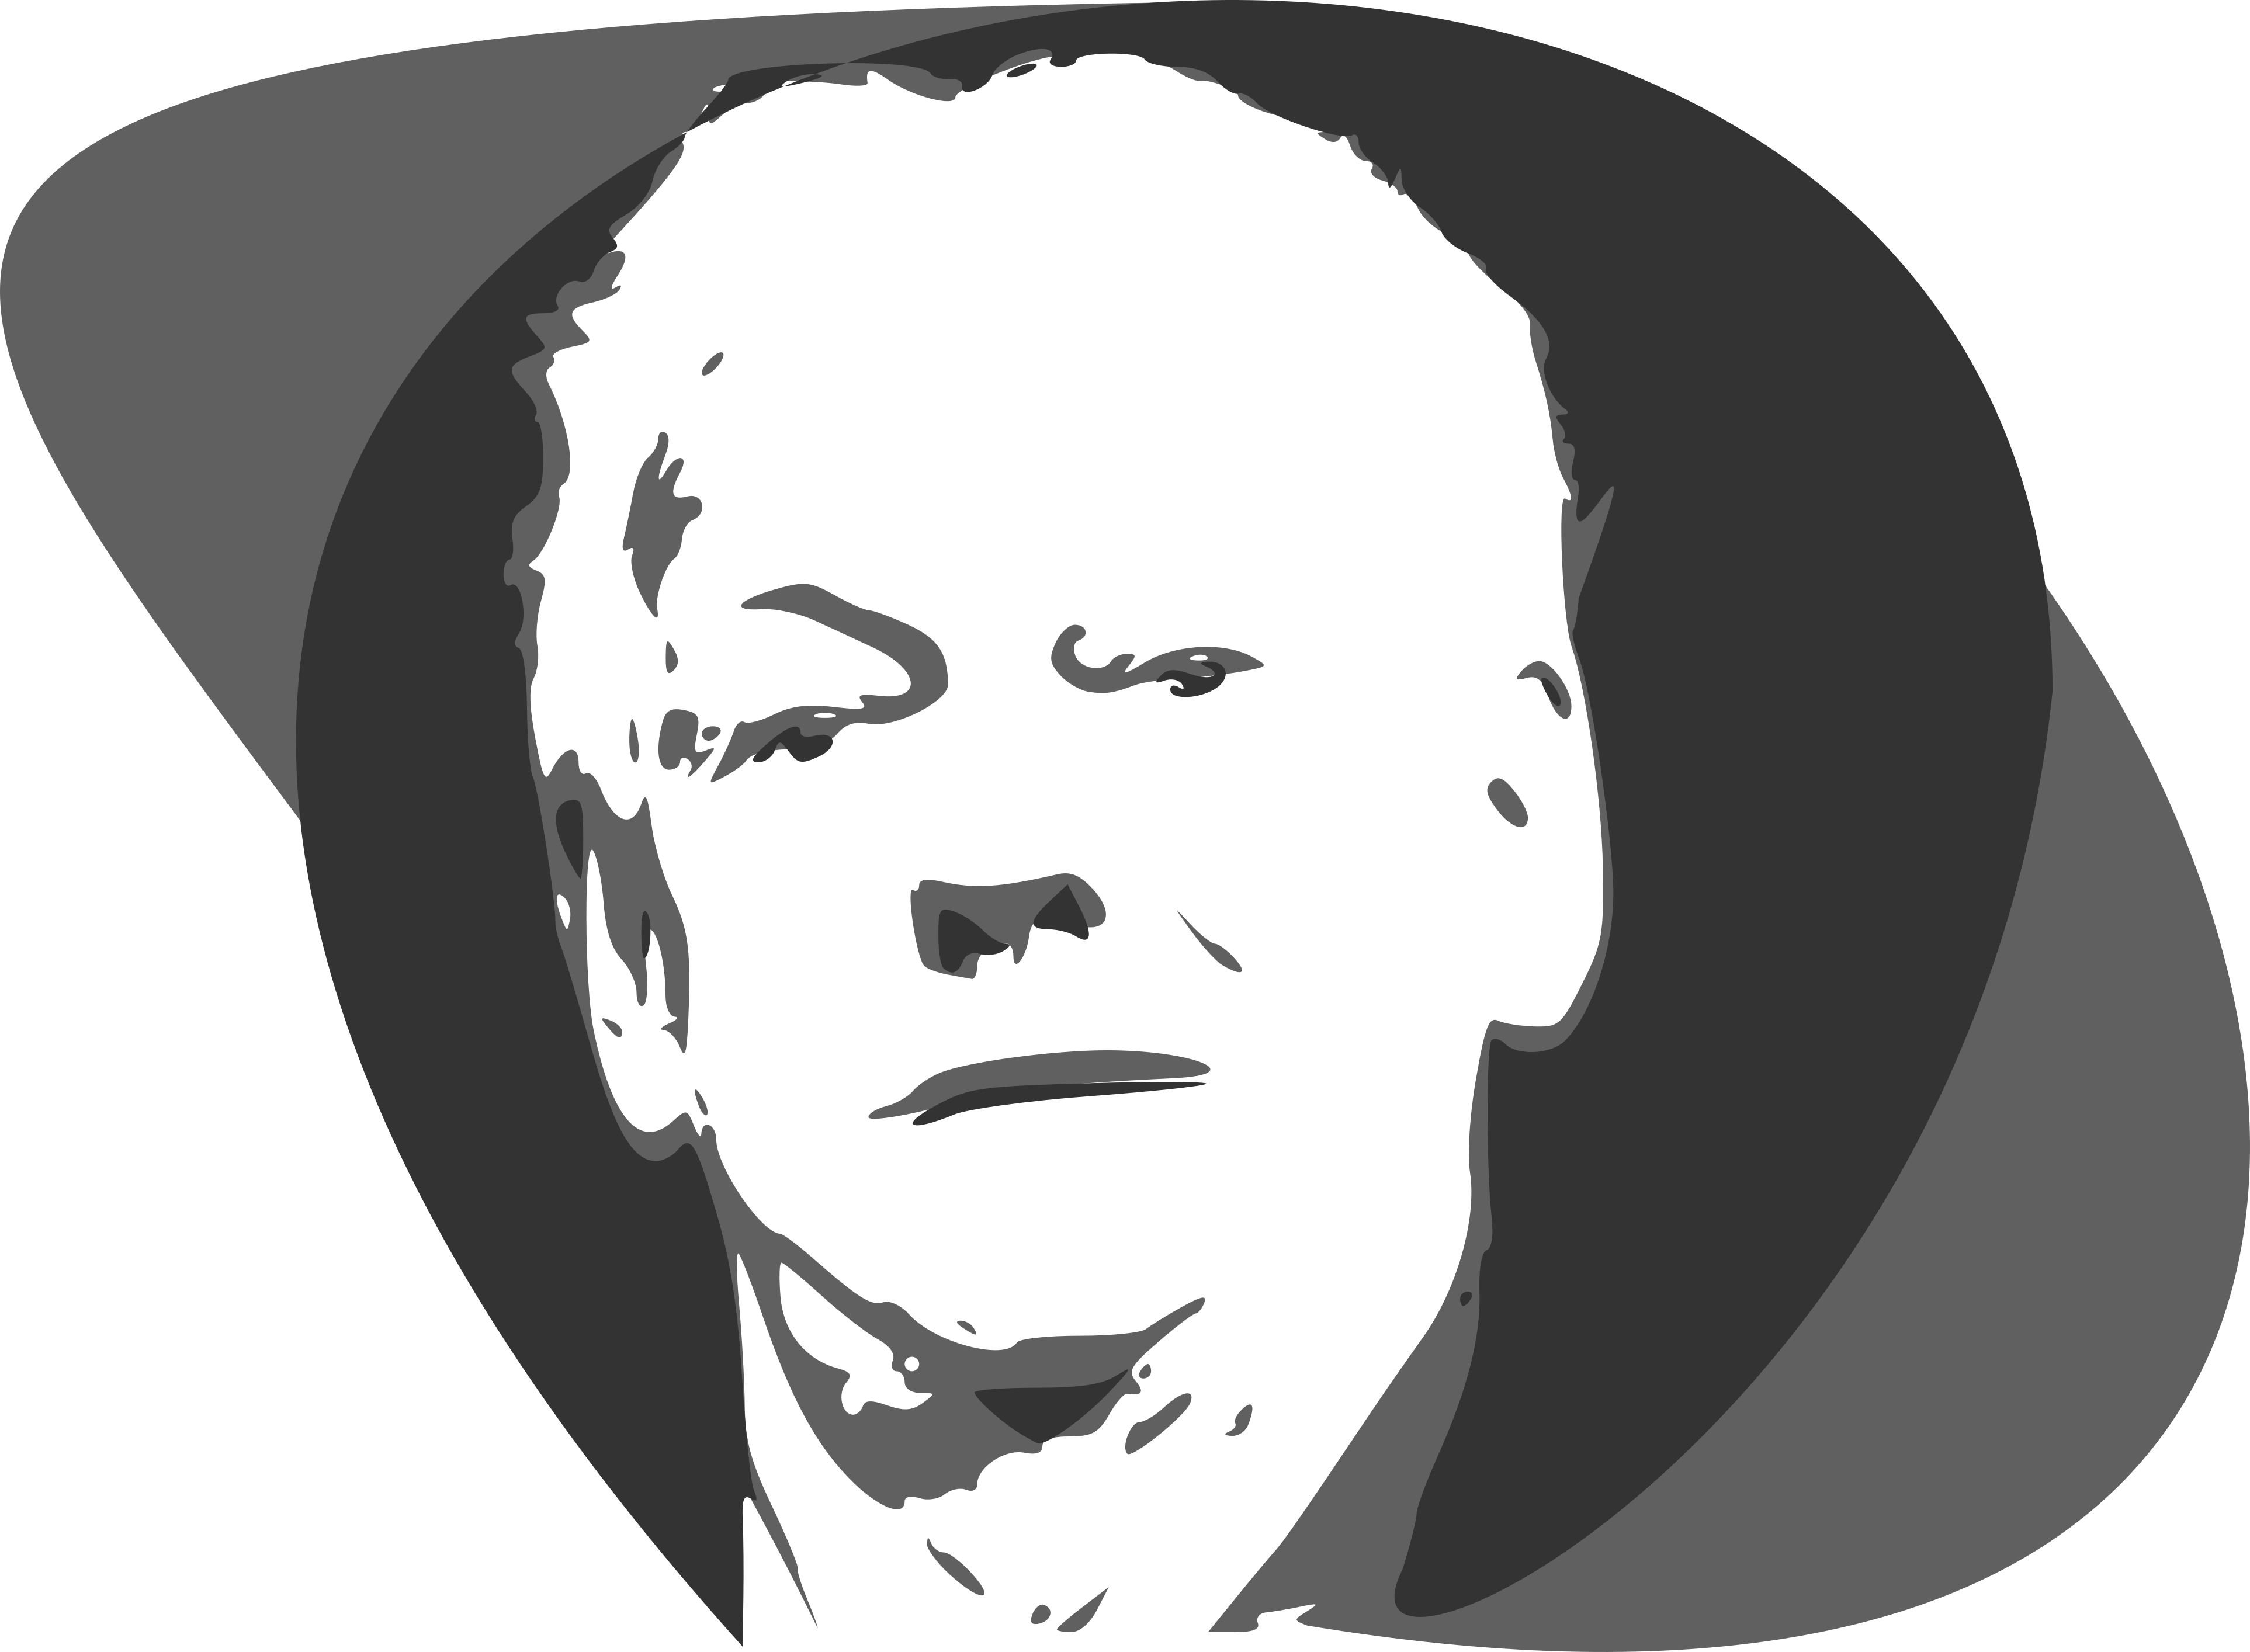
\includegraphics[width=\textwidth]{./bilder/wheterby.png}
\end{center}
\vspace*{\fill}
{\centering\fontsize{50}{48} \color{farbe}\sffamily{Wheterby Castle}\par}
\addcontentsline{toc}{chapter}{Wheterby Castle}
\newpage
%%%%%%%%%%%%%%%%%%%%%%%%%%%%%%%%%%%%%%%%%%%%%%%%%%%%%%%%%%%%%%%%%%%%%%%%%%%%%%%
\lettrine[lines=3, lhang=.2, loversize=.25, lraise=0.05, findent=0.1em,
nindent=0em]{D}{ie} Fahrt von London hat neun Stunden gedauert. Der Smog der Stadt geht fliessend in den Nebel vom Land über. Landschaft von nicht mehr als 20 Yard. Zugschwellen genen den Rythmus vor, verbieten jeden Gedanken. Tristesse und Trance im überhitzten Abteil. Von York aus nehme ich eine Kutsche in Richtung Küste. Schlaglöcher machen den Körper taub. Ich sollte für Lady Cantacuziono in London ein Stadthaus kaufen. Eine verwitwete rumänische Adlige, transsilvanischer Hochadel, sehr reich, mehr weiss ich nicht über sie. Ich habe einige Vorschläge, verschiedene Villen, ein kleines Schloss, Wohnungen in Kensington. Nachdem Geschäft sollte endlich das Gelfür die lange versprochenen Flitterwochen am Meer übrig sein. Die Hochzeit ist schon zwei Jahre her, die Erinnerung durch Alltag verblasst.

Der Kutscher bekreuzigt sich, als ich die Adresse nenne. \enquote{Seid ihr Christ? Dann nehmt dieses Kreuz.}, und reicht mir eine Kette, die fast ein Rosenkranz ist. \enquote{Das Haus ist verflucht, man sagt, dass alle die dort gewesen sind, entweder wahnsinnig wurden oder ganz verschwunden sind, überlegt es Euch gut, mein Herr.} 

Geschwätz mochte ich nie, Vorurteile kann ich mir nicht leisten. Es ist später Nachmittag als ich ankomme. Ein herrliches Schloss, historisierend gothisch, aber neu. \enquote{Sie hat einen Friedhof geschändet.} brummt der Fuhrwerker, Prim ausspuckend, brauner Schleim im Matsch. \enquote{Nun ja, nicht wirklich, aber Grabsteine für ertrunkene Seeleute haben hier gestanden, damit die Hinterbliebenen einen Ort zum Trauern haben. Ins Meer hat sie die geworfen.} Ihn ignorierend höre ich tatsächlich die See branden, tief unten an der Steilküste. Möwen schreien. Wenn ich das Meer sehe, habe ich Fernweh, schmecke Salz in der Luft. Kühler Wind, nicht stark, aber der Kraft, Armeen von Schiffen zu tragen. Mich an London erinnern, dessen Russ und Schmutz ich so liebe, ist hier unmöglich. Die Kutsche verschwindet im Nebel, mich alleine lassend.

Das schwere Tor ist geöffnet, der Garten wild, viele Rosen, in Hecken, als Büsche, rankend, blühend, verwelkt. Auf mein Klopfen reagiert niemand. \enquote{He}, rufe ich. Also stosse ich die Tür selber auf, trete ein, beklommen, ein Eindringling. Dabei sollte der Brief, der mich angekündigt hat, bereits hier sein. Ein grosser Saal, ein grosser Tisch, gedeckt für eine Person. Schweres Holz, Alter vortäuschend, als wäre es schon immer da gewesen. Gemälde bereits Verstorbener, Goldketten trangend, Zepter zur Schau stellend, Herschaflichkeit ausstrahelnd. Womit haben sie verdient, hier zu hämgen, was zeichnet sie aus?


Ein Zettel \enquote{Esst, ich stosse später zu Euch.}. Kaltes Huhn, fast roh, aber die Kartoffeln heiss und dampfend. Warum keine Bediensteten? Es ist unheimlich, ich schäme mich meiner, fühle mich falsch. Die Stille ist kaum zu ertragen. Aber die Reise war ermüdend, Hunger egalisiert anderes. Also esse ich. Der Wein ist fast schwarz, schmeckt tief und schwer, scheint sich im Hals aufzulösen, wird den Magen nie erreichen. Der beste, den ich je getrunken habe. In einem Zug leere ich den silbernen Becher, kann nicht absetzen.

\enquote{Ihr habt geschlafen.} Tatsächlich, meine Verwirrung ist vollkommen. Ich muss während des Essens eingeschlafen sein, warum erinnere ich mich an nichts? Das Huhn steht immer noch beinahe unagetastet vor mir. Es ist bereits dunkel, Kerzen erleuchten das Zimmer nur matt. Daher sehe ich sie nicht gleich, reibe mir verstört die Augen, aber noch steckt zu viel Schlaf in ihnen, um Schärfe zu erlauben.

\enquote{Willkommen auf Whetherby Castle. Ich bin Lady Cantacuziono.} Das Kreuz des Kutschers ist verschwunden, ich weiss es ohne in die Tasche zu greifen. Sie ist ganz in schwarz gekleidet, in tiefem Kontrast zu ihrer prozellanweissen Haut. Das Gesicht ist nicht zu erkennen. Seltsam langsame Bewegungen, fast verträumt. Sie nimmt eine Nuss aus einer Schale, umschliesst sie mit zarten Fingern und knackt sie, als wäre dies die natürlichste Art. Wie die Nuss in ihren Mund gelangt, verstehe ich nicht.

\enquote{Ich habe sie erwartet}. Ich stehe endlich auf, erschrocken von meiner Unhöflichkeit, verbeuge mich, gebe ihr die Hand. Wie kalt sie ist. Ich erkläre mich, stammele wie peinlich mir es sei, eingeschlafen zu sein, mit einer angedeuteten Geste deutet sie mir aufzuhören. Ich spüre wie mir Schweiss den Rücken herabläuft, bin verlegen, verunsichert.

\enquote{Wenn sie wünschen kann ich ihnen gerne die Unterlagen geben, ich habe verschiedene Optionen für sie ausgewählt\dots} 

\enquote{Sie werden mir ein Haus kaufen, ich bin an Optionen nicht interessiert.}, weist sie mich zurück. Sagt sie das wirklich oder meine ich es nur zu hören? Es muss an diesem Schlaf liegen, der nicht verschwinden will, aber warum kann ich die Frau nur undeutlich sehen? Mein Blick verschwimmt, aber nur bei Ihr. Den fetten Mann auf dem riesigen Bild sehe ich, Goldene Knöpfe auf der Brust,aber sie? Wie der Rauch einer erlöschenden Kerze.

\enquote{Erlauben sie mir eine Frage}, setze ich an, will wissen, warum es keine Diener gibt, weswegen ich mich so eigenartig fühle, aber sie verneint bevor ich die Frage stellen kann mit einer Geste, die ich nicht kenne aber verstehe. Pachuli. Ein schwerer Geruch umströmt sie, wird mir jetzt bewusst, erreicht mich, dringt auch in mich ein. Ich muss endlich aufhören zu träumen, muss mich fokussieren, kann es aber nicht. Werde immer tiefer hinabgezogen. Sand zerrieselt zwischen meinen Fingern. Ich entschuldige mich stotternd, versuche die Fassung zu wahren. War sie eben auch schon so riesig? Sie scheint den Raum vollständig auszufüllen, ist dabei aber weiter zerbrechlich zart, elegant. Ihr Anblick verweht, wenn ich ihn fassen will, sie ist überall und doch nicht da. Ich spüre ihre glatte und zarte Haut.

Ich stütze mich auf den Tisch, der Schweiss tropft mir aus den Haaren, wie finde ich mich wieder? Sie führt mich in ein Zimmer, ich schlottere, kann mir nicht helfen. Dass sie mir zwei riesige Hunde zu meinem Schutz da lässt, nehme ich nicht wahr. Gross und drohend sitzen sie vor meinem Bett, in das ich sinke ohne die Kleider zu wechseln. Sie werden die ganze Nacht knurren und am Morgen verschwunden sein. Ich schlafe nicht, träume nur. Der einzige Mitgefangene in meinem kleinen Kerker ist meine Angst. Schwarz und kalt. Einsamkeit, Verlassensein, Leere. Als endlich die Sonne aufgeht stehe ich auf, bin wieder alleine in dem Schloss. Die Nacht ist vorbei, ich weiss wieder wer ich bin, was ich bin. 

Ein unterschriebener Kaufvertrag liegt auf dem Tisch, von draussen ruft ein Kutscher.\hfill \pgfornament[color=farbe,height=.5cm]{3}
\newpage 


\thispagestyle{empty}
\begin{center}
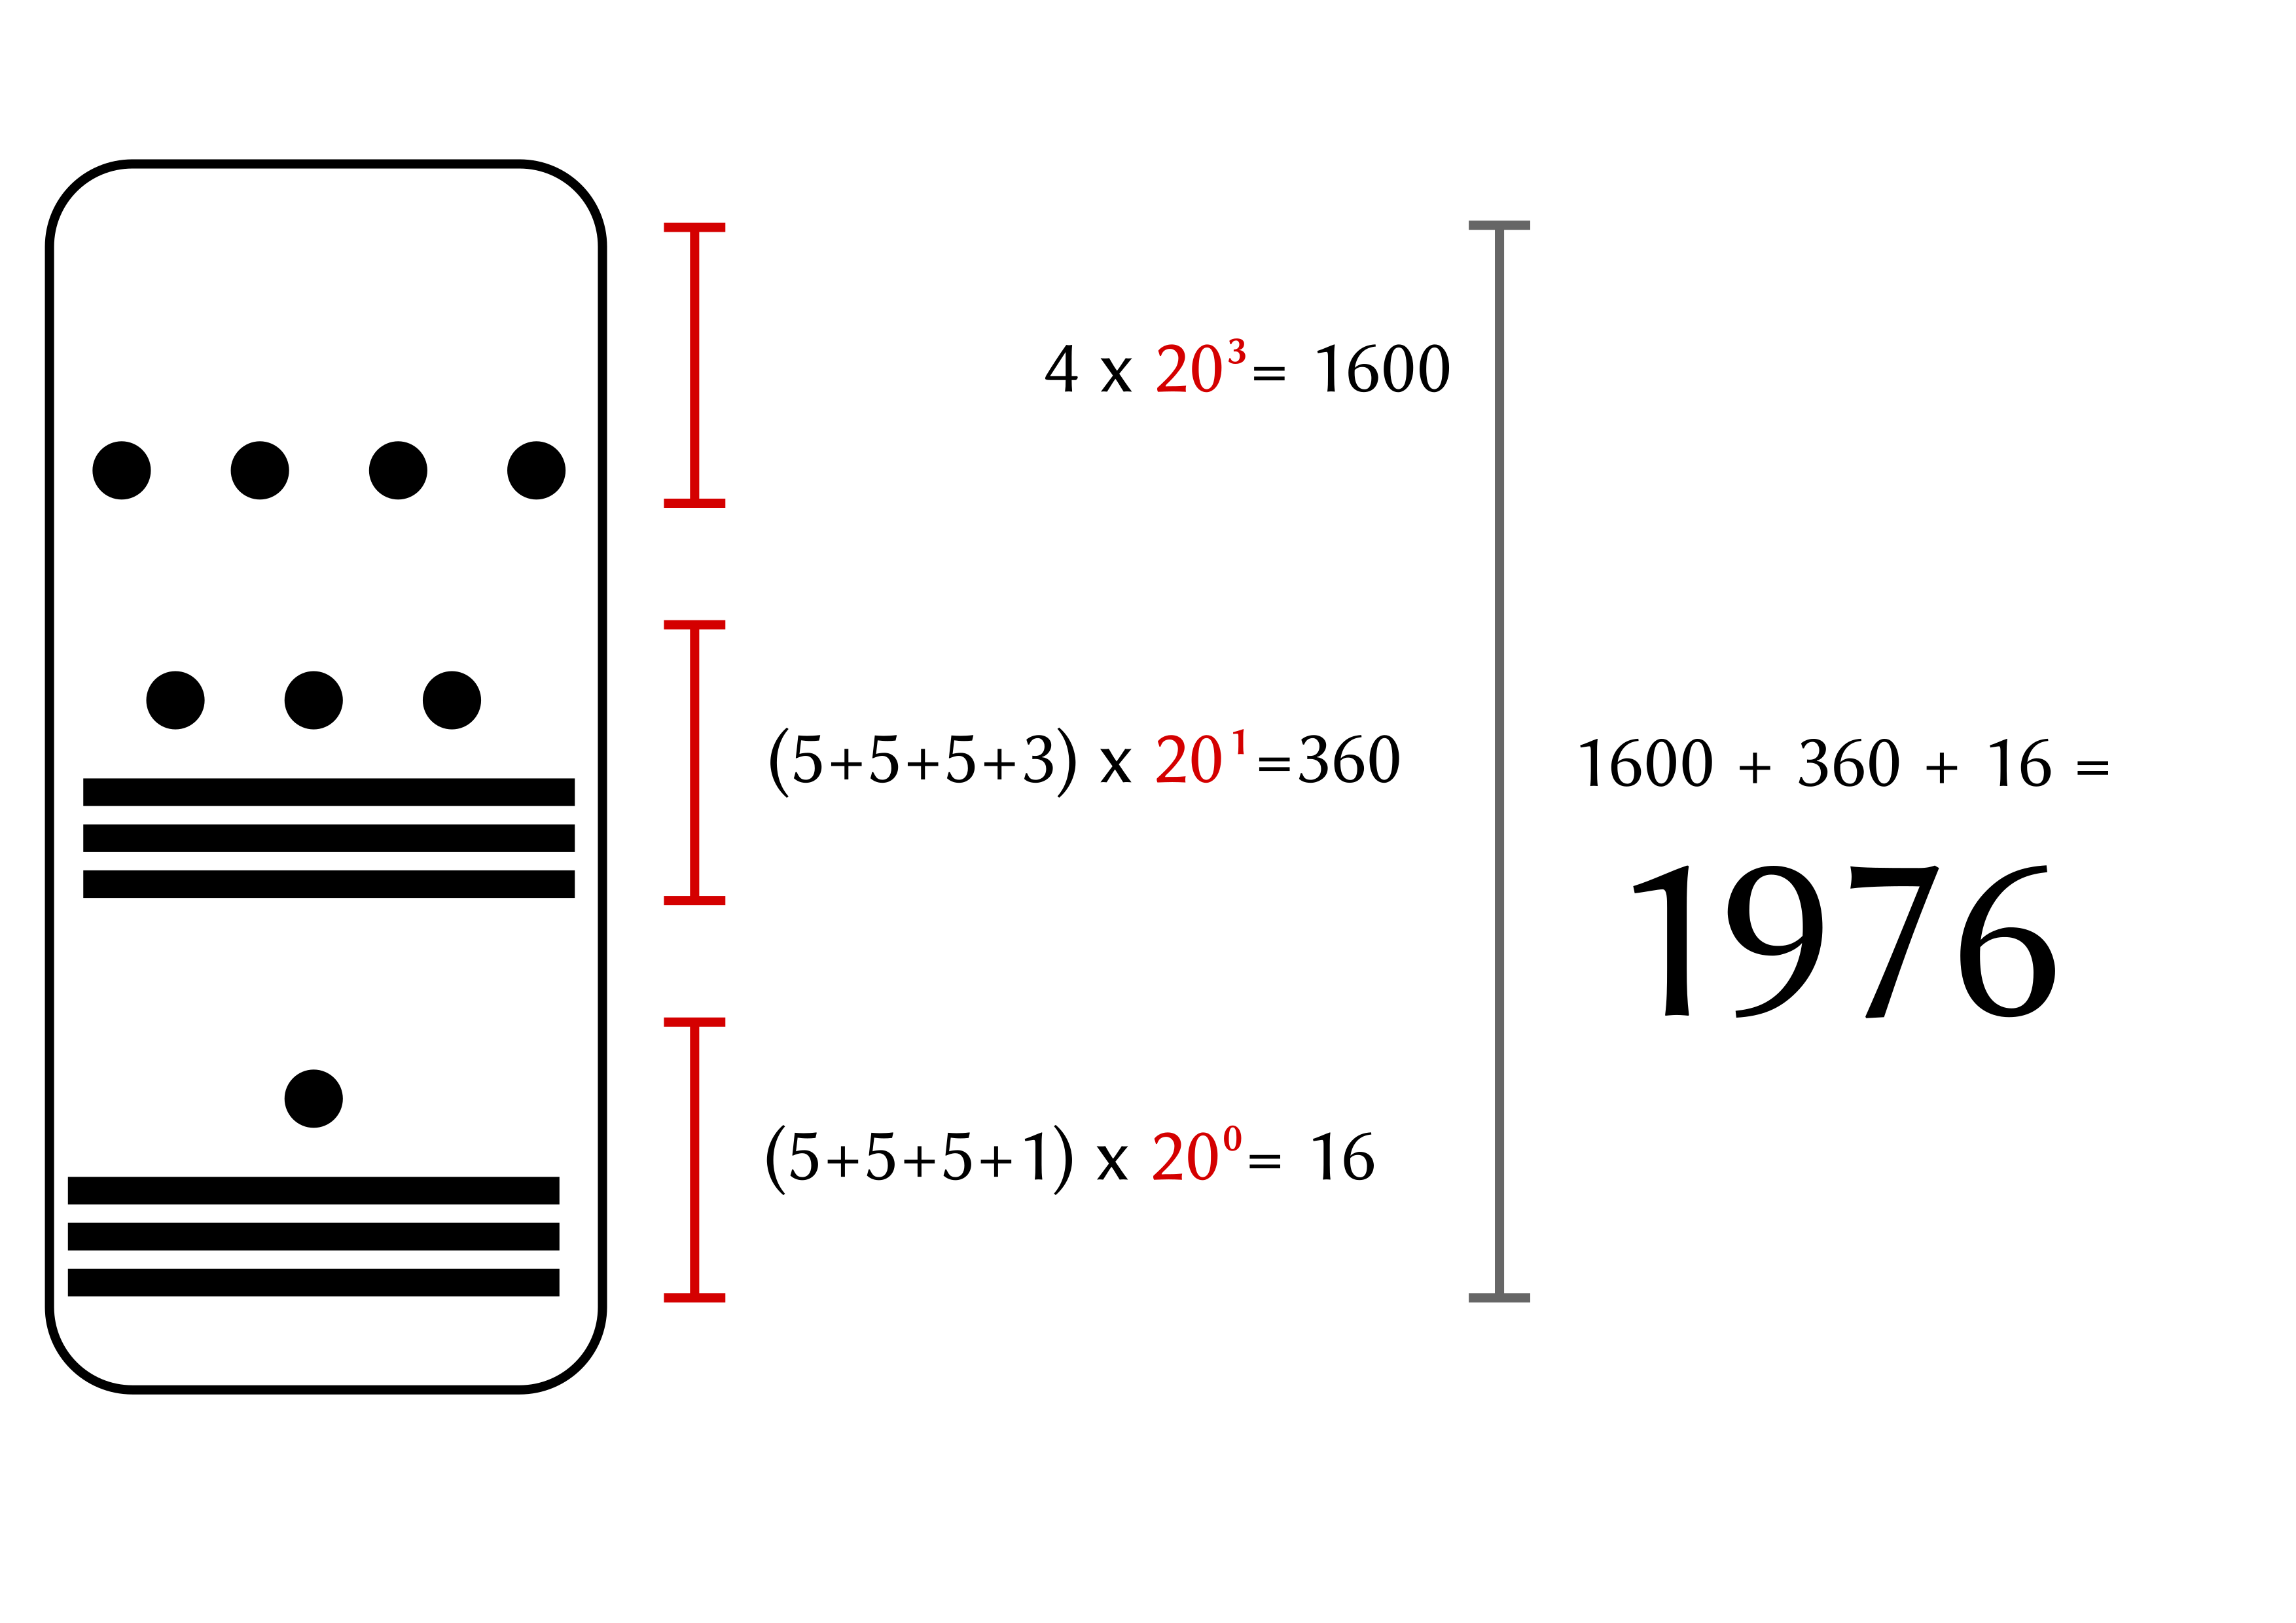
\includegraphics[width=\textwidth]{./bilder/Maya1976.png}
\end{center}
\vspace*{\fill}
%{\Huge\color{farbe}\hfill{\ttfamily{Fangen}}}
{\centering\fontsize{50}{48} \color{farbe}\sffamily{Zahlen und Ziffern}\par}
\addcontentsline{toc}{chapter}{Zahlen und Ziffern}
\newpage
%%%%%%%%%%%%%%%%%%%%%%%%%%%%%%%%%%%%%%%%%%%%%%%%%%%%%%%%%%%%%%%%%%%%%%%%%%%%%%%
\lettrine[lines=3, lhang=.2, loversize=.25, lraise=0.05, findent=0.1em,nindent=0em]{A}{ls} wir die Geschichte \enquote{Acht} in diesem Buch geschrieben haben, haben wir anstelle von Namen Ziffern verwendet. Ein wie ich finde hübscher Einfall von Paula, der funktioniert. Aber warum tut er das? Warum ist es möglich, dass sofort klar ist, dass das Zeichen \Circled{8} etwas wie ein Name sein soll? Die Antwort ist, dass wir hier mit dem Unterschied zwischen Ziffern und Zahlen gespielt haben. Wenn Du 8 liest, hast du etwas sehr Kompliziertes im Kopf, wofür die Menschheit sehr lange gebraucht, es zu erfinden, du siehst die Zahl. Mittlerweile können Mathematikerinnen zwar erklären, was eine Zahl ist, das ist aber sehr verwirrend und kompliziert.

Zahlen haben nichts damit zu tun, wie man sie schreibt oder darstellt. Da haben verschiedene Kulturen verschiedene Lösungen gefunden, die mal mehr und mal weniger tauglich sind, Schülerinnen das Rechnen beizubringen. Ein paar davon möchte ich dir hier vorstellen.

Aber vorher nochmals zurück zu den Zahlen. Zahlen sind universell, das heisst, die Regeln, denen sie folgen gelten überall und immer. Warum weiss niemand, aber das Wort \enquote{universell} darfst du wörtlich verstehen. Wenn es Ausserirdische geben sollte --wovon ich übrigens aus rein mathematischen Überlegungen ausgehe-- und wir irgendwann einmal Kontakt mit ihnen haben, sollte unsere Mathematik und die der Ausserirdischen dieselbe sein, auch wenn sie sonst vielleicht mit Lichtblitzen statt mit Schallwellen kommunizieren.

Das gilt auch auf der Erde. Egal welche Sprache du sprichst, Mathematik funktioniert immer. Nicht, dass irgendjemand die gesamte Mathematik versteht, aber es sollte möglich sein, jemanden zu finden, der intelligent genug ist, den Bereich zu verstehen und zu beweisen, ob das was mit Mathematik gesagt wurde, richtig ist oder falsch. Ganz präzise.

Ein Beispiel für Mathematik. Die folgenden Überlegungen sind ganz unabhängig von den Ziffern. Du spielst mit Legosteinen, alle sehen gleich aus und bestehen aus zwei Reihen mit je vier von diesen Noppen\footnote{Dieser 4x2 Stein ist übrigens der klassischste aller Legosteine. Er ist massstäblich einem echten Backstein nachempfunden. Alle anderen Legosteine leiten ihre Grösse genau von diesem Stein ab.}. Und Du hast jetzt ein paar Steine davon und willst wissen, wie viele mögliche Figuren du damit bauen kannst, das heisst du fragst dich, auf wie viele verschiedene Arten du die Steine verbinden kannst. Natürlich werden nicht alle Kombinationen schön aussehen, aber vielleicht interessiert dich doch die Frage, wie viele Dinge du mit deinen Steinen bauen könntest.

Dann hilft dir Mathematik und die gilt, egal ob du eigentlich Schweizerdeutsch, Französisch oder $!$X\'{o}\~{o} sprichst\footnote{Die Sprache ǃ X\'{o}\~{o} heisst tatsächlich so! Sie wird auch Taa genannt und gehört zu den Tuu Sprachen. Sie wird in Botswana und Namibia gesprochen, allerdings nur noch von sehr wenigen Menschen. Das Besondere ist, dass sie sehr viele Laute enthält, insgesamt 159. Man bräuchte also 159 verschiedene Buchstaben oder Buchstabenkombinationen wie im Deutschen \textit{sch} um alle Laute zu schreiben. Such mal im Internet nach der Sprache. 83 Laute sind Schnalz- und Klicklaute. Für unsere Ohren klingt das sehr spannend!}. Aber wie so oft üblich, müssen wir erst einmal eine Einschränkung machen. Wir sehen uns nur Kombinationen an, bei der die Steine entweder parallel oder im rechten Winkel zueinander sind. Steine \textit{schief} aneinander zu bauen, ist nicht erlaubt, dann wäre die Lösung schon bei zwei Steinen unendlich. Die Formel zu Berechnung der Anzahl möglicher Kombinationen lautet:

$$2^{n-1}+\frac{46^{n-1}-2^{n-1}}{2}$$

Oha! Wer soll denn das verstehen? Aber es ist weniger schwierig las du denkst, lass dich von der Schreibweise nicht abschrecken! Rechnen wir es doch mal an einem Beispiel durch. Sagen wir, du hast nur zwei Steine zur Verfügung. überleg erst einmal selbst im Kopf, wie du beide Steine kombinieren kannst.

Und jetzt lass uns kurz rechnen. $n$ ist die Anzahl der Steine, die du zur Verfügung hast. Im Beispiel gilt also $n=2$. Jetzt setzen wir die 2 in die Gleichung ein. Wie du vielleicht schon aus der Schule weisst, bedeutet die Schreibweise, wenn etwas hochgestellt ist, auch \textit{hoch} oder besser ausgedrückt, Potenz. $2^3$ heisst nichts anderes, als dass wir $2\times2\times2$ rechnen. Probieren wir das doch mal mit dem ersten Stück (Term genannt) der Gleichung aus und rechnen $2^{2-1}=2^1=2$ Okay. Dazu addieren wir den zweiten Term, den wir stückweise ausrechnen. Beginnen wir über dem Bruchstrich. $46^{2-1}=46$. Davon ziehen wir wieder die bereits bekannten $2^{2-1}=2$ ab und kommen auf 44. Der Bruchstrich ist nichts anderes als ein \textit{geteilt durch das was unten steht}, also $2$. Die Lösung für zwei Steine ist, dass es $24$ verschiedene Kombinationen gibt.

Das verrückte an dieser Formel ist, die Lösung wächst unglaublich schnell, das bedeutet, dass die Anzahl möglicher Kombinationen sehr schnell sehr gross wird, wenn du nur wenige Steine hinzunimmst. Die Anzahl Kombinationen beträgt zum Beispiel für 6 legosteine $915'103’765$ also fast eine Milliarde. Probiere es aus, wenn du es nicht glaubst! Wenn Du allerdings je Kombination sagen wir 10 Sekunden benötigst, wirst du 290 Jahre Tag und Nacht beschäftigt sein. Eine langweilige Idee, nehme ich an. Bei 25 Steinen beträgt die Anzahl Kombinationen

\begin{footnotesize}
$$4'028'635'400'867'168'454'517'798'790'018'457'665’536$$
\end{footnotesize}

Eine bizarr grosse Zahl! Viel mehr weiss man nicht, die Zahlen, die danach folgen, sind schlicht zu gross, um berechnet zu werden. Für 47 Lego-Steine bräuchte der beste Computer (Stand 2005) 130 Jahre. Nein halt, ganz falsch, er bräuchte eine Anzahl Jahre, bei der auf die 130 noch 39 Nullen folgen! Keine Chance in diesem Universum.

So kann man also verschiedenste Dinge mit Hilfe der Mathematik beschreiben und verstehen. Mit Mathematik könnten wir uns also auch mit Ausserirdischen über Lego unterhalten. Würde mich doch sehr wundern, wenn die nicht etwas Ähnliches bei sich haben. Aber es gibt auch einen Teil, der eben nicht gleich ist auf der Welt und das sind die Ziffern. Ziffern ist die Art, wie du Zahlen schreibst, welche Zeichen und welches System du verwendest. Mit System meine ich übrigens den logischen Aufbau der Ziffern, dazu komme ich gleich noch.

Die Unterschiede zwischen den Kulturen betreffen nicht nur die Art, wie die Ziffern geschrieben werden, sondern auch, wie sie benannt werden. Damit meine ich nicht den reinen Wortlaut wie \textit{zwei} auf Hochdeutsch, \textit{two} auf Englisch oder \textit{$\neq$n\^{u}m} auf $!$X\'{o}\~{o}. Wie man das Zeichen $\neq$ wohl auspricht? --sondern wie die Wörter für die Zahlen aufgebaut sind. Jetzt kommt etwas sehr Kompliziertes, das du vermutlich noch nicht verstehst. Mathematik beschäftigt sich mit dem Wert der Zahlen. Und dabei spielt es keine Rolle, wie die Zahlen geschrieben oder benannt werden. Das wird durch die Kultur und gelegentlich praktischen Gründen bestimmt.

Wir verwenden indisch-arabischen Ziffern, die haben sich in Indien aus der Brahmi-Schrift (3. Jahrhundert vor Christus, aber die Angaben gehen auseinander) entwickelt. Das betrifft weniger die Zeichen selbst, aber auch, sondern vor allem das System. Als endgültige Geburtsstunde gilt jedenfalls das Jahr 628, als ein Mann namens Brahmagupta die Null als vollwertige Zahl etabliert hatte. Da das System ziemlich gut funktioniert hat, hat es sich von da ab schnell ausgebreitet und auch die arabische Welt erreicht, die es über den Umweg Nordafrika auch in Europa populär gemacht haben. Das war dan naber erst im 13. Jahrhundert.

Aber was fanden denn die Leute damals so cool an dem System? Es verwendet nur zehn Zeichen (Glyphen ist das Angeberwort dazu) und ist streng logisch aufgebaut. Das System funktioniert nämlich ganz einfach: wenn du immer grössere Zahlen schreiben willst, fängst du zunächst mit den zehn einfachen Zeichen:

$$0, 1, 2, 3, 4, 5, 6, 7, 8, 9$$
Du musst dir nur zehn Zeichen merken und ihre Reihenfolge. Aber ab Zehn gehen dir die Zeichen aus, und du willst keine neuen hinzunehmen (weil das sonst nicht cool wäre, habe ich ja gerade gesagt). Aber funktionieren würde es schon. Man könnte ja zum Beispiel sagen, dass $\Theta$ Elf, $\Xi$ Zwölf und so weiter bedeuten könnte und so könnten wir uns für jede Zahl ein eigenes Zeichen ausdenken. Das ist aber nicht nur für dich schwer zu merken, gerade wenn du manche Zahlen nur selten benutzt, wie die wirklich blöde siebenundachtzig. Also belässt du es bei den zehn Zeichen und wendest einen genialen Trick an. Sobald dir die Zeichen ausgehen, setzten du beginnend mit dem kleinsten Zeichen nach der 0 dieses vorne dran und beginnst hinten wieder von vorne von unten nach oben die bekannten Zeichen zu verwenden. Nach $\dots, 8, 9,\dots$ kommt der Sprung $\dots, 10, 12, 13, 14,\dots$

Und wenn du dann wieder ans Ende gekommen bist, nimmst du vorne das nächste Zeichen und fängst da an hochzuzählen: $\dots, 18, 19$ und dann Zack $20, 21, 22,\dots$ und wenn dir dann wieder die Zeichen ausgehen, setzen du wieder eine Ziffer vorne dran, nach $\dots, 98, 99$ geht es weiter mit $100, 101,102\dots$. Alles sehr schön logisch und unkompliziert. Damit kannst du leicht und verständlich beliebig grosse Zahlen schreiben.

Und dann hat diese Schreibweise den Vorteil, dass sie sogar noch leicht erweiterbar ist, wenn du nämlich Zahlen schreiben willst (oder eher musst) die zum Beispiel grösser als $1$, aber kleiner als $2$ sind. Dann setzt man nämlich ein Komma (oder wie hier in der Schweiz und vielen anderen Ländern üblich einen Punkt) hinter die letzte volle Zahl und kann dann den sogenannten gebrochenen Teil weiterschreiben. Versuch mal da mit eigenen Worten zu erklären, wie die Regel funktioniert und warum zum Beispiel $4.5$ grösser ist als $4.42$.

Die verwendeten Zeichen können sich natürlich je nach Schrift unterscheiden, das System bleibt aber in den meisten Sprachen dasselbe. Hier ein paar, die mir gefallen (manchmal steht an der Stelle der Null das Zeichen für 10):

\begin{center}
\small
\begin{tabular}{ c c c c c c c c c c l}
0 & 1 & 2 & 3 & 4 & 5 & 6 & 7 & 8 & 9 & {\tiny Hindu-Arabisch}\\
\FontC{௦} & \FontC{௧} & \FontC{௨} & \FontC{௩} & \FontC{௪} & \FontC{௫} & \FontC{௬} & \FontC{௭} & \FontC{௮} & \FontC{௯} & {\tiny Tamil}\\
\FontD{0} & \FontD{๑} & \FontD{๒} & \FontD{๓} & \FontD{๔} & \FontD{๕} & \FontD{๖} & \FontD{๗} & \FontD{๘} & \FontD{๙} & {\tiny Thai}\\
\FontE{ი} & \FontE{ა} & \FontE{ბ} & \FontE{გ} & \FontE{დ} & \FontE{ე} & \FontE{ვ} & \FontE{ზ} & \FontE{ჱ} & \FontE{თ} & {\tiny Georgisch}\\
\FontF{०} & \FontF{१} & \FontF{२} & \FontF{३} & \FontF{४} & \FontF{५} & \FontF{६} & \FontF{७} & \FontF{८} & \FontF{९} & {\tiny Devanagari}\\
\FontG{十} & \FontG{一} & \FontG{二} & \FontG{三} & \FontG{四} & \FontG{五} & \FontG{六} & \FontG{七} & \FontG{八} & \FontG{九} & {\tiny Japanisch}\\
\FontB{י} & \FontB{א} & \FontB{ב} & \FontB{ג} & \FontB{ד} & \FontB{ה} & \FontB{ו} & \FontB{ז} & \FontB{ח} & \FontB{ט} & {\tiny Hebräisch}\\
\FontH{٠} & \FontH{١} & \FontH{٢} & \FontH{٣} & \FontH{٤} & \FontH{٥} & \FontH{٦} & \FontH{٧} & \FontH{٨} & \FontH{٩} & {\tiny Arabisch}\\
\FontI{ꊰ} &\FontI{ꋍ} & \FontI{ꑍ} & \FontI{ꌕ} & \FontI{ꇖ} & \FontI{ꉬ} & \FontI{ꃘ} & \FontI{ꏃ} & \FontI{ꉆ} & \FontI{ꈞ} & {\tiny Yi}\\
\end{tabular}
\end{center}
Die Mathematik hat sich seit Erfindung dieses Systems immer weiterentwickelt und wie die meisten Wissenschaften in den letzten wenigen hundert Jahren rasant. Das hat es nötig gemacht, die Schreibung von Zahlen auf viele Arten zu erweitern. Beispielsweise ist schon ganz früh klar gewesen, dass sich ein Drittel nicht ohne weiteres mit diesem System schreiben lässt, da müsstest du unendlich viele Dreien schreiben, womit du spätestens aufhören müsstest, wenn jemand \enquote{Zähneputzen} ruft. Schon in der Antike haben die Griechen zeigen können, dass das auch für $\sqrt{2}$ gilt. Sie gehört übrigens zur Gruppe der irrationalen Zahlen. Hinzu kamen negative Zahlen (mit einem Minus gekennzeichnet) und dann so verrückte Dinge wie irrationale Zahlen die man mit einem $i$ schreibt und manche Zahlen, die auch nicht gutgeschrieben werden können, haben dann doch noch ein eigenes Zeichen bekommen, wie die berühmte Kreiszahl $\Pi$.

Das System, Zahlen so aufzubauen, lässt sich übrigens leicht variieren. Warum zum Beispiel ausgerechnet zehn verschiedene Symbole? Na ja, die einfache Antwort ist wohl, dass die meisten Menschen zehn Finger haben und unser Zählen als Kind damit beginnt. Aber das ist nicht immer das einfachste. Ein Computer funktioniert so, dass er eigentlich nur zwischen \textit{da fliesst gerade Strom} und \textit{da fliesst gerade kein Strom} unterscheiden kann. Dann kannst du dir den Speicher des Computers ganz vereinfacht vorstellen als viele Punkte, an denen entweder eben Strom fliesst oder eben nicht. Wenn wir jetzt Strom fliesst mit dem Symbol $1$ bezeichnen und kein Strom mit $0$, können wir Zahlen in einem sogenannten Binärystem, also mit lediglich zwei Zeichen schreiben. Die Logik bleibt dieselbe:

\begin{small}
\begin{center}
\begin{tabular}{ c c l }
0 & 0 & die ersten beiden Zahlen sind noch gleich\\
1 & 1 & ab der 1 fehlen uns aber weitere Zeichen \\
2 & 10 & also fügen wir vorne wieder eine an \\
3 & 11 & unten hinter wieder weiterzählen\\
& & Ach schon wieder fertig?\\
&& Also wieder vorne eine dazu\dots \\
4 & 100 & und so weiter bis Unendlich.
\end{tabular}
\end{center}
\end{small}
Manchmal werden im Computer (auf einer anderen Eben, das ist hier aber egal) auch sogenannte Hexadezimalzahlen eingesetzt. Das System verwendet 16 verschiedene Zeichen, nach der $9$ folgt $A$, als elf dann $B$ und so weiter bis fünfzehn als $F$. Das Hexadezimalsystem wird verwendet, da man somit die Leistung des Computers optimal nutzen kann. Wieso genau sei jetzt mal egal\footnote{Ich habe zwar versucht, zu erklären warum das so ist, aber nicht geschafft, es in einfache Worte zu bringen. Da lass ich es doch einfach weg. Frag mich, wenn es dich interessiert.}. Ein anderes Beispiel ist das Zahlensystem der Maya (die früher in Mexiko gelebt haben). Sie hatten als Basis die zwanzig. Ihre Ziffern waren so aufgebaut

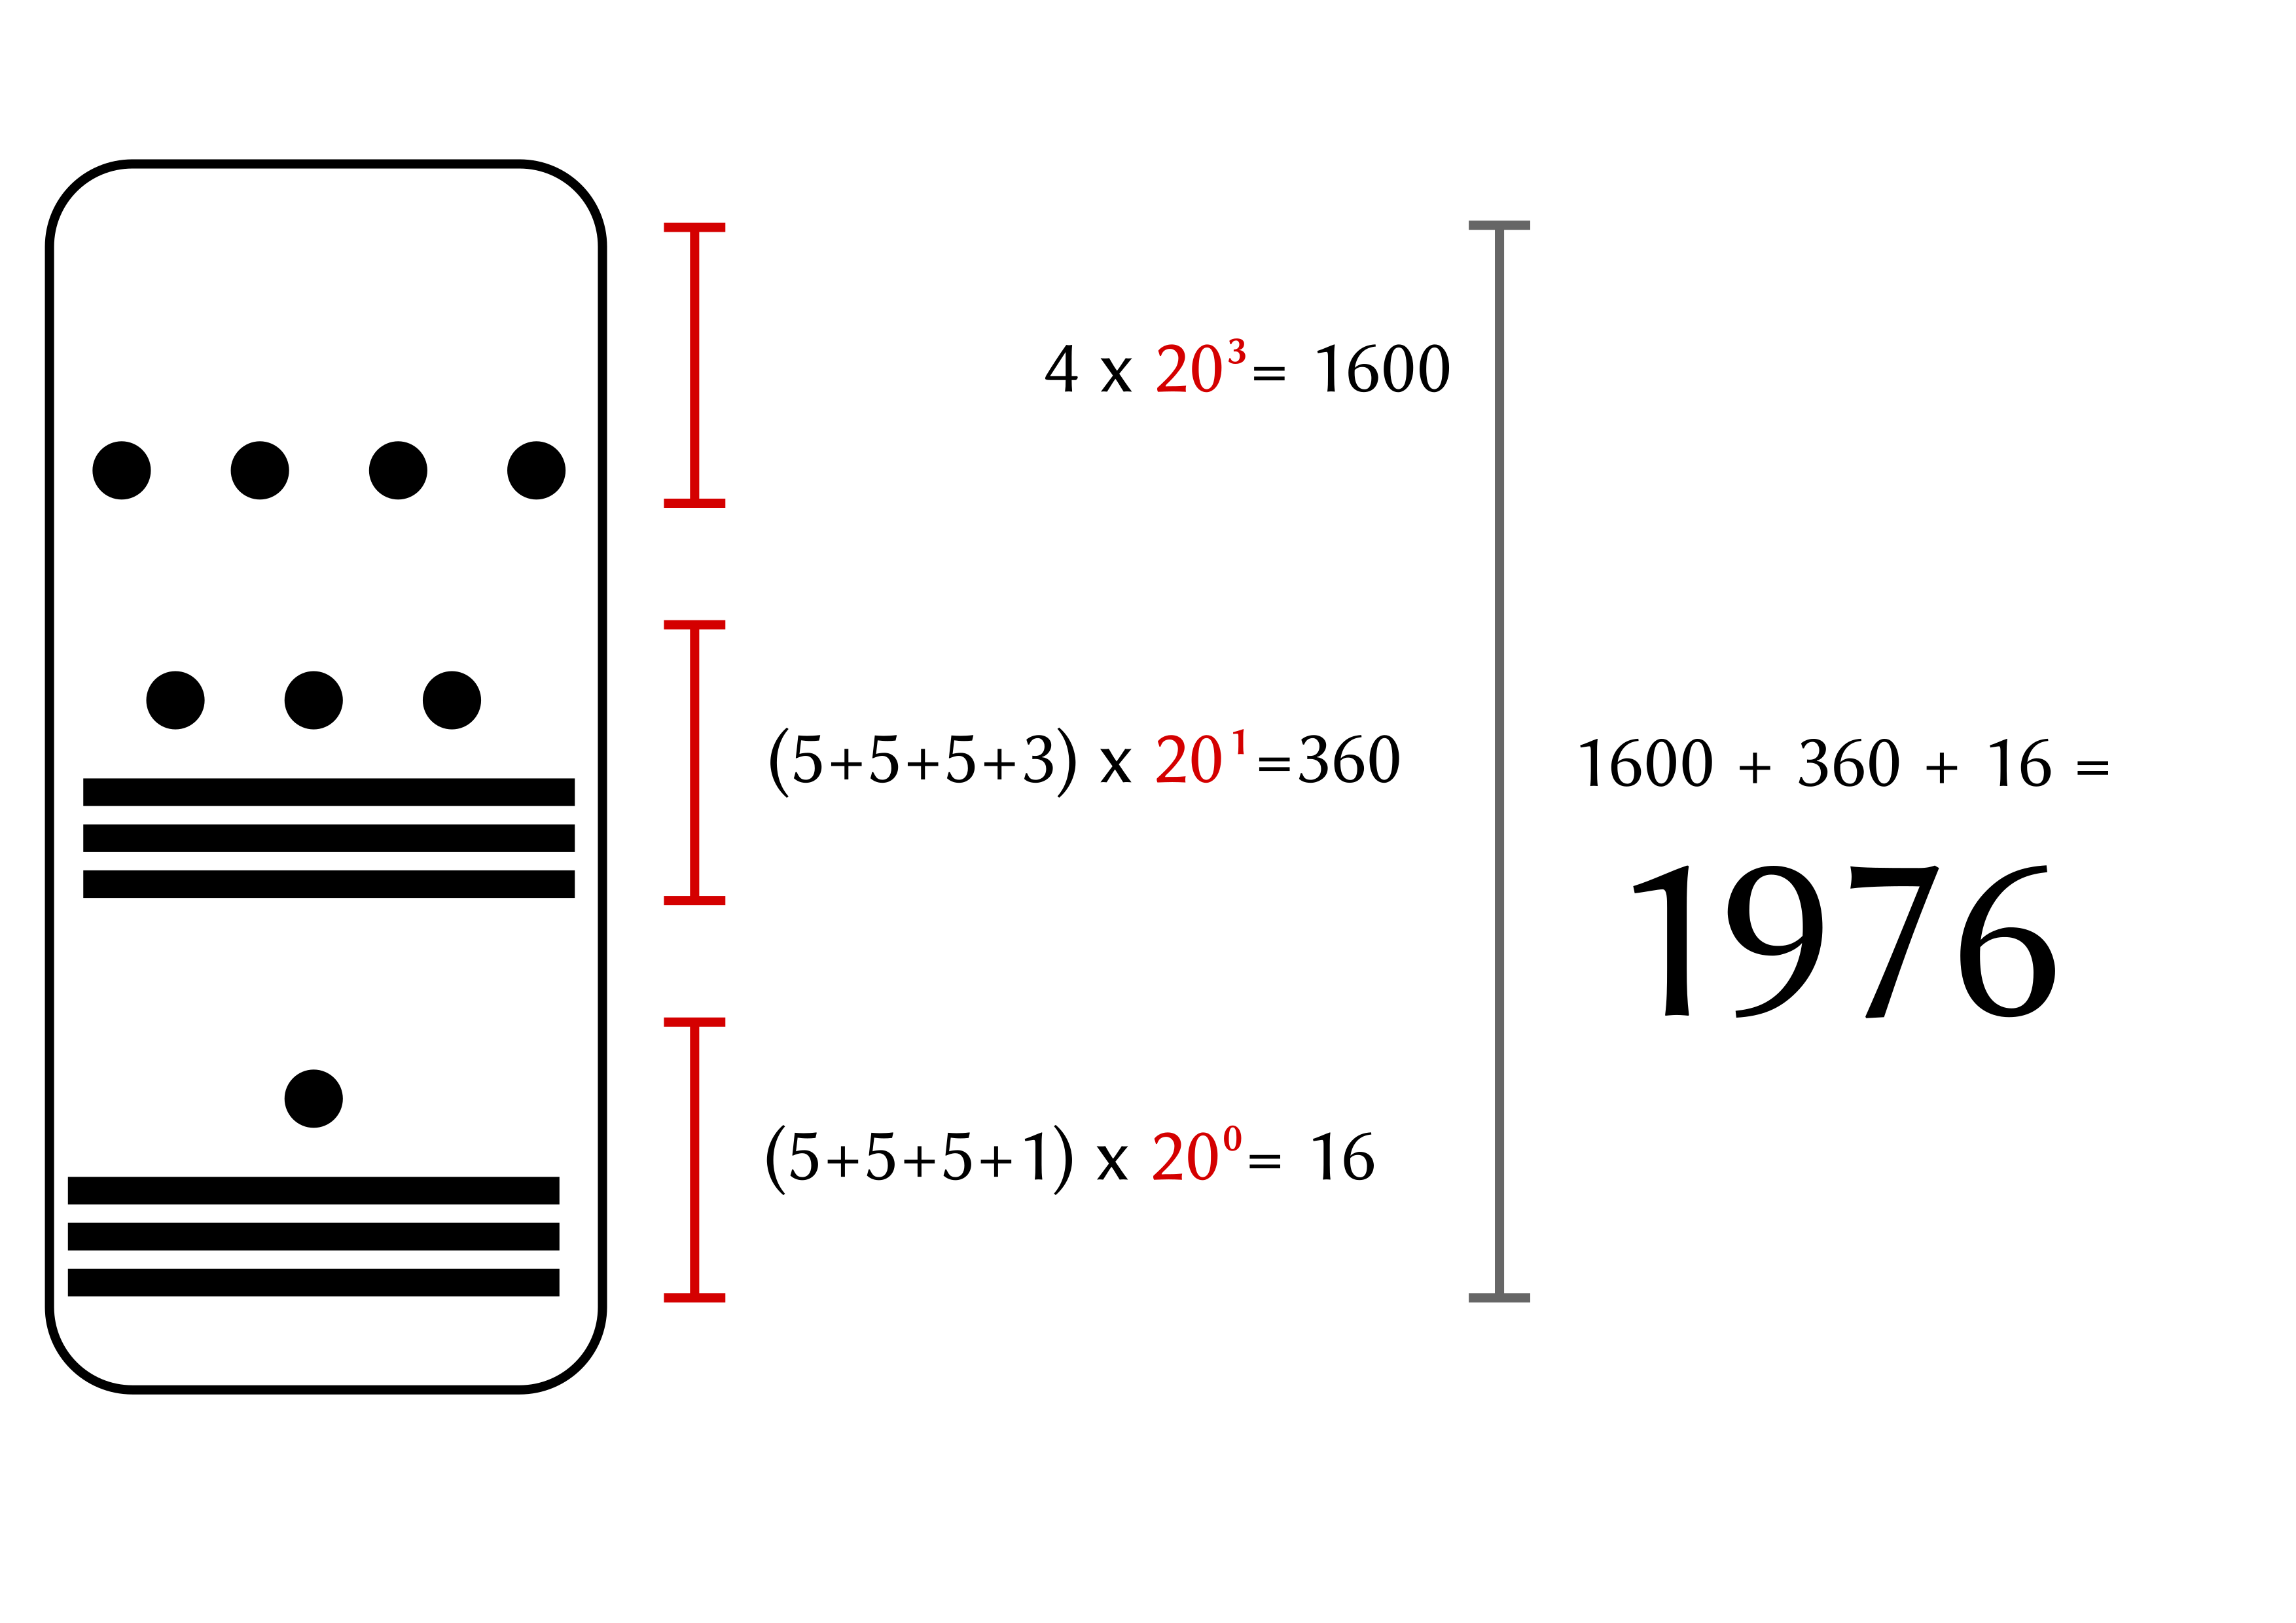
\includegraphics[width=\textwidth]{./bilder/Maya1976.png}

Und es gibt noch viel mehr Möglichkeiten, Zahlen zu schreiben, die sich aber nicht bewährt haben.

Die einfachste und erste Methode wird Unärsystem genannt und ist schon mindestens 50'000 Jahre alt. Um sich das Rechnen zu erleichtern, haben Menschen damals einfach Kerben in ein Stück Holz oder einen Knochen geritzt. Die Menschen haben also zunächst nur ein Zeichen verwendet, nämlich einen Strich |. Und dann lautet die Regel zur Bildung der Zahlen einfach, dass sie das Zeichen so oft wiederholen mussten, bis es dem gewünschten Wert entsprach. 13 schreibt man also einfach als |||||||||||||.

Das ist sehr mühsam und kann leicht zu Verwechslungen führen. Daher hat man angefangen, die Striche zu gruppieren. Aus der Bronzezeit sind zum Beispiel Ägäische Zahlzeichen überliefert. Dort sahen die ersten zehn Zahlen so aus:
%%%%%%%%%%%%%%%%%%%%%Hier einfügen

Genau wie bei dieser Schrift hat man auch im alten Ägypten gewisse Anzahlen von Strichen zusammengefasst und ein neues Zeichen (Hieroglyphe) vergeben. Insgesamt gab es sechs verschiedene:

1 \textpmhg{\Hone}, 10 \textpmhg{2}, 100 \textpmhg{3}, 1’000 \textpmhg{4}, 10’000 \textpmhg{5}, 100’000 \textpmhg{6}, 1'000’000 \textpmhg{7}. Cäsar und die anderen im alten Rom haben dann, wenn auch wesentlich später, eine ähnliche Idee gehabt. Du kennst die römischen Ziffern sicher aus einem Asterixheft. In dem lauten Tumult der Märkten damals hat man sich oft mit Zeichensprache unterhalten. Aus zwei gekreuzten Fingern für zehn, ist dann das X geworden und für fünf, der Hälfte der Zehn hat man halt auch das halbe Zeichen verwendet, das V. Aber die schlaueste Art Zahlen zu schreiben, war das nicht. Die Null zu schreiben ging zum Beispiel gar nicht und grosse Zahlen waren sehr mühsam. Aber über viele Jahrhunderte hatte man hier in Europa keine bessere Idee, bis endlich die indisch-arabischen Ziffern eingeführt wurden.

Jetzt könnte man meinen, dass wir die Zahlen auch so nennen, wie sie geschrieben werden. Bei vielen Zahlen trifft das im Deutschen zu: $17$ also siebzehn setzt sich auch sprachlich zusammen aus \textit{sieben} und \textit{zehn}. Das passt oft. Ausnahmen sind die Elf und die Zwölf. Vor allem die Zwölf war früher, als man Dinge noch auf dem Markt eingekauft hat, eine wichtige Zahl, weil sie durch so viele andere teilbar ist, nämlich der 2, 3, 4, und 6. Das geht mit 10 nicht. Weil sie so gut teilbar ist, verwenden wir sie auch noch bei der Uhrzeit bei den Stunden und als Vielfaches von fünf, also 60 bei den Minuten. Man kann so bequem ausrechnen, wie viele Minuten eine Viertelstunde hat. Und ich nehme an, weil die Zwölf so wichtig war, hat sie einen echten eigenen Namen verdient und da musste die Elf natürlich dann auch noch einen bekommen.

Wo es sprachlich leider im Deutschen dann doch etwas durcheinandergeht, sind grössere Zahlen. Zum Beispiel wird die $135’782$ als \textit{einhundert fünf und dreissig tausend sieben hundert und zwei und achtzig} ausgesprochen. Sehr blöd. Wir nennen zuerst die erste Stelle, dann die Dritte, dann die Zweite, dann die Vierte, dann die letzte und dann die Vorletzte. Wer auf so einen Unfug wohl gekommen ist?

Aber das Problem ist in anderen Sprachen noch schlimmer. Für dich am bekanntesten ist sicher Französisch. Zum Beispiel heisst 97 \textit{quatre-vingt-dix-sept} als wörtlich übersetzt \textit{Vier (mal) Zwanzig (plus) Zehn (plus) Sieben}. Ernsthaft? Noch verrückter wird es im Dänischen. Dort scheint irgendetwas gründlich schief gelaufen zu sein. Die ja eigentlich sehr häufig verwendete Zahl 50 heisst \textit{halvtredsindstyvende}, was wörtlich übersetzt \textit{(Drei minus ein Halb) mal Zwanzig} bedeutet. Schnell nachrechnen: $3-0.5=2.5$ und $2.5\times20=\dots$ Musik spielt im Hintergrund solange mein Hirn sich quält $\dots = 50$ Stimmt, bleibt aber sehr sonderbar!

Was dir vielleicht aufgefallen ist, ist das sowohl im Dänischen, wie auch im Französischen die zwanzig eine Rolle spielt. Das macht sie in vielen Kulturen. Es könnte zwei Erklärungen dafür geben: entweder werden die Zehen beim Rechnen zu den Fingern hinzugenommen, oder diese einfach umgedreht.

Dieses sogenannte Vigesimalsystem findet man in Afrika, Asien und an vielen anderen Orten. Es ist noch nicht lange her, da hat man in England 20 Schillinge zu einem Pfund zusammengefasst. Am weitesten verbreitet war das System bei den Maya im heutigen Mexiko. Ein Bild dazu hast du ja weiter oben schon gesehen. Die Maya haben Nahuatl gesprochen, eine Sprache, die es selbst heute noch gibt\footnote{Ganz unbekannt ist dir die Sprache nicht, denn Wörter wie Tomate, Schokolade und Kakao haben wir auch im Deutschen aus Nahuatl übernommen.}. In Nahuatl leiten sich die Namen der ersten fünf Zahlen von \textit{Hand} und die nächsten fünf von \textit{entgegengesetzter Hand} ab. Das Wort für zwanzig heisst in Quiché, einer anderen Maya-Sprache k‘hal, was \textit{ganzer Mensch} bedeutet, also im Sinne von mit Fingern und Zehen. In einigen ostafrikanischen Sprachen ist das auch so.

Unser Körper bestimmt unser Zahlensystem. Da wundert es mich doch, dass in der Welt der Simpsons auch ein 10er-Zahlensystem existiert, auch wenn dort alle nur vier Finger an jeder Hand haben. Wenn du dich übrigens geschickt anstellst und das Prinzip kennst, kannst du mit den Händen locker bis 59‘048 zählen. Es geht sogar noch höher, wenn du gelenkig bist. Such das mal im Internet, das Prinzip ist verblüffend. Auch heute noch wird auf manchen Märkten mit solchen Techniken gezählt, das nennt man irritierenderweise \enquote{Frauenrechnen} oder \enquote{Arithmetik aus Marseille}.

In wieder anderen Sprachen gibt es nur wenige Wörter für Zahlen. Das aus unserer Sicht wohl skurrilste Beispiel ist die Sprache der Piraha, das ist ein Volk, das im brasilianischen Amazonasgebiet lebt. Die kennen nur drei Zahlen: \textit{eins}, \textit{zwei} und \textit{viele}. Verwirrenderweise kommt noch hinzu, dass das Wort für \textit{eins} dasselbe ist wie für \textit{zwei}, bloss anders betont. Noch verwirrender ist, dass \textit{eins} auch \enquote{ungefähr eins} und zwei \enquote{nicht viele} bedeuten kann. Nicht nur, dass die keine Wörter für Zahlen haben, es fällt ihnen auch schwer, mit einer Anzahl umzugehen. In einem Test wurden ihnen eine gewisse Anzahl Früchte gegeben, zum Beispiel zehn, und sie sollten gleichviele hinzulegen oder die Anzahl mit den Fingern zeigen. Das hat bei den meisten nicht geklappt, jedenfalls nicht mehr bei mehr als drei Früchten! Es gibt also auch ein Leben ohne Zahlen, aber aus Sicht der restlichen Menschheit ist das schon sehr selten. Ich meine damit auch gar nicht, dass die Leute dort dumm sind, Zahlen und Zählen ist einfach nur kein Teil ihrer Kultur.

Was nebenbei bemerkt spannend ist, dass ähnliche Tests auch mit Tieren gemacht wurden. Wie die genau gemacht wurden, sollte man sich vielleicht nochmals ansehen, ich habe keine Ahnung, ob das wirklich stimmen kann. Jedenfalls gilt aktuell, dass Schimpanzen demnach mindestens bis neun zählen können, viele Vögel bis sieben, Ameisen bis 20 und Ratten sogar bis 24. Mit Zählen ist gemeint, dass sie die Anzahl abschätzen können, sie haben natürlich kein Wort oder hübsches Zeichen dafür, ausser vielleicht Papageie, aber die würden es gar nicht merken. Kinder in unserem Kulturraum schaffen den Test bis zehn typischerweise im Alter von drei Jahren.

Zum Schluss noch zwei kleine Spielereien, sogenannte numerische Palindrome, die ausschliesslich nur funktionieren, weil wir das Dezimalsystem haben. 
\begin{equation*}
\begin{aligned}
1\times9 + 2 &= 11\\
12\times9 + 3 &= 111\\
123\times9 + 4 &= 1111\\
1234\times9 + 5&= 11111\\
12345\times9 + 6 &= 111111\\
123456\times9 + 7 &= 1111111\\
1234567\times9 + 8 &= 11111111\\
12345678\times9 + 9 &= 111111111\\
\end{aligned}
\end{equation*}

\begin{equation*}
\begin{aligned}
1\times1 &= 1\\
11\times11 &= 121\\
111\times111 &= 12321\\
1111\times1111 &= 1234321\\
11111\times11111 &= 123454321\\
111111\times111111 &= 12345654321\\
1111111\times1111111 &= 1234567654321\\
11111111\times11111111 &= 123456787654321\\
111111111\times111111111 &= 12345678987654321
\end{aligned}
\end{equation*}
\hfill \pgfornament[color=farbe,height=.5cm]{3}

\newpage


\thispagestyle{empty}
\begin{center}
\includegraphics[width=\textwidth]{./bilder/drache.png}
\end{center}
\vspace*{\fill}
%{\Huge\color{farbe}\hfill{\ttfamily{Fangen}}}
{\centering\fontsize{50}{48} \color{farbe}\sffamily{Der Drache}\par}
\addcontentsline{toc}{chapter}{Der Drache}
\newpage
%%%%%%%%%%%%%%%%%%%%%%%%%%%%%%%%%%%%%%%%%%%%%%%%%%%%%%%%%%%%%%%%%%%%%%%%%%%%%%%
\lettrine[lines=3, lhang=.2, loversize=.25, lraise=0.05, findent=0.1em,
nindent=0em]{I}{ch} bin der Zerstörer, das Biest, der Schlächter. Der Drachen. Mein Herr hat mich gekauft, für 100 Sesterzen. Ich bin ein teuerer Sklave. Der Teuerste in diesem Ludum. Verschont beim Training. Fleisch schon am Morgen. Wurde gehegt. Salben aus den südlichen Provinzen, um die Blutungen zu stillen. Aber nicht für mich, sondern für solche Augenblicke.

Die Arena. Jubel. Extase. Tod. Ich töte. Ich bin Gladiator. Sklave um Sklaven zu töten. Besitz, Wert, Ware zerstören für Jubel. Ihr Schreien ist mein Lohn, meines Herren Gold, das, was mir erlaubt zu leben.  

Dafür töte ich. Nehme anderes Leben, das keines mehr ist. Er oder ich. So einfach. Klar. Exakt. Endgültig. Ich bin kein Mensch und wäre ich es wirklich nicht, hätten sie keinen Spass. Ich bin Macht. Zeige, dass wir aus Blut bestehen. Im Sand bleibt es, auch wenn die Körper längst entsorgt sind. 

Gleich wird sich das Gitter wieder heben. Und mit ihm der Jubel. Zu Ehren welcher Gottheit ich heute kämpfen werde, töte oder sterbe, weiss ich nicht. Es sind nicht meine Götter, sondern die meines Herren. Mein Atem ist laut im Helm. Ich werde eins mit ihm. So lange ich atme, lebe ich. 

Ich habe Angst. Ich habe Wut. Aber beide verschwimmen vor meiner Lust zu kämpfen. Und zu töten. Sieger zu sein. Ich. Nicht der Thraker. Siegen ist ein nicht endender Rausch. Alles erreichen, das Schlimmste ist vermieden. Nichts ist grösser, intensiver, lebendiger. Alles Leben wird mich umschlingen, wenn seines endet. 

Das Gitter hebt sich. Sand unter meinen Sandalen. Zwei Schritte. Dann rennen. Schwert und Schild verlieren Gewicht, werden Teil meines Körpers. Fliegen. Mein Schrei vor mir. Verkündet mich. Ich komme, Thraker.  \hfill \pgfornament[color=farbe,height=.5cm]{3}
\newpage
 


%%%%%%%%%%%%%%%%%%%%%%%%%%%%%%%%%%%%%%%%%%%%%%%%%%%%%%%%%%%%%%%%%%%%%%%%%%%%%%%%%%%%%%%%%%%%%%%%%%%%%%
%Inhaltsverzeichnis
\newpage
\pagestyle{empty}
\tableofcontents

\end{document}
